\documentclass[12pt]{article}

% Packages
\usepackage[utf8]{inputenc}
\usepackage{xcolor}
\usepackage{titlesec}
\usepackage[margin=1in]{geometry}
\usepackage{graphicx}
\usepackage{float}
\usepackage{indentfirst}
\usepackage{subcaption}

% Define section blue
\definecolor{myblue}{RGB}{0, 102, 204}

% Set section colors
\titleformat{\section}
  {\color{myblue}\normalfont\Large\bfseries}
  {\thesection}{1em}{}

\titleformat{\subsection}
  {\color{myblue}\normalfont\large\bfseries}
  {\thesubsection}{1em}{}

% Document info
\title{\textbf{Using Bayesian Optimization On The Suzuki Coupling Reaction}}
\author{Marlow Lichty and Miguel Angel Cisneros\\
Institute for Computing in Research, Santa Fe, New Mexico}
\date{\color{myblue}\bfseries\today}

\begin{document}

\maketitle

\section{Abstract}

In this project, we explored the use of Bayesian Optimization to improve reaction discovery using the EDBO (Experimental Design via Bayesian Optimization) repository. We updated the repository’s dependencies and refactored parts of the code to being our work, including replacing the original Jupyter notebook files with Marimo notebooks. After, we looked around for datasets with yield data to test reaction optimization as we had no lab to test experiments in. Eventually settling on a dataset for the Suzuki coupling reaction, we modified the model parameters and gave the model different features until we were able to identify high-yielding conditions in far fewer steps than the original experimental workflow of the dataset. 

\section{Introduction}
Optimizing chemical reactions takes a lot of trial and error, which costs time, money, and materials. The Suzuki coupling is one of the most widely used reactions in organic chemistry, especially in pharmaceuticals, but finding the best combination of base, solvent, ligand, and catalyst can be overwhelming without help. That’s where tools like Bayesian Optimization come in, they’re designed to search smarter instead of just trying every possible combination.

For this project, we used a tool called EDBO (Experimental Design via Bayesian Optimization) to see how well it could suggest good reaction conditions. We didn’t have access to a lab, and even if we did, four weeks wouldn’t be enough to run the number of experiments we’d need. So instead, we worked with reaction data and focused on fixing up the code, finding better datasets, and testing how EDBO performs when given limited information. Our goal was to see if BO could help predict better reaction setups and do it faster than traditional methods.

\section{Background}
The Suzuki coupling reaction is a widely used method in organic chemistry that forms carbon–carbon bonds. It involves a reaction between a nucleophile (usually a boronic acid) and an electrophile (often an aryl halide) in the presence of a palladium catalyst, a base, and a solvent. It’s especially popular in pharmaceutical research because it’s reliable, flexible, and works with a lot of different functional groups.

\begin{figure}[H]
    \centering
    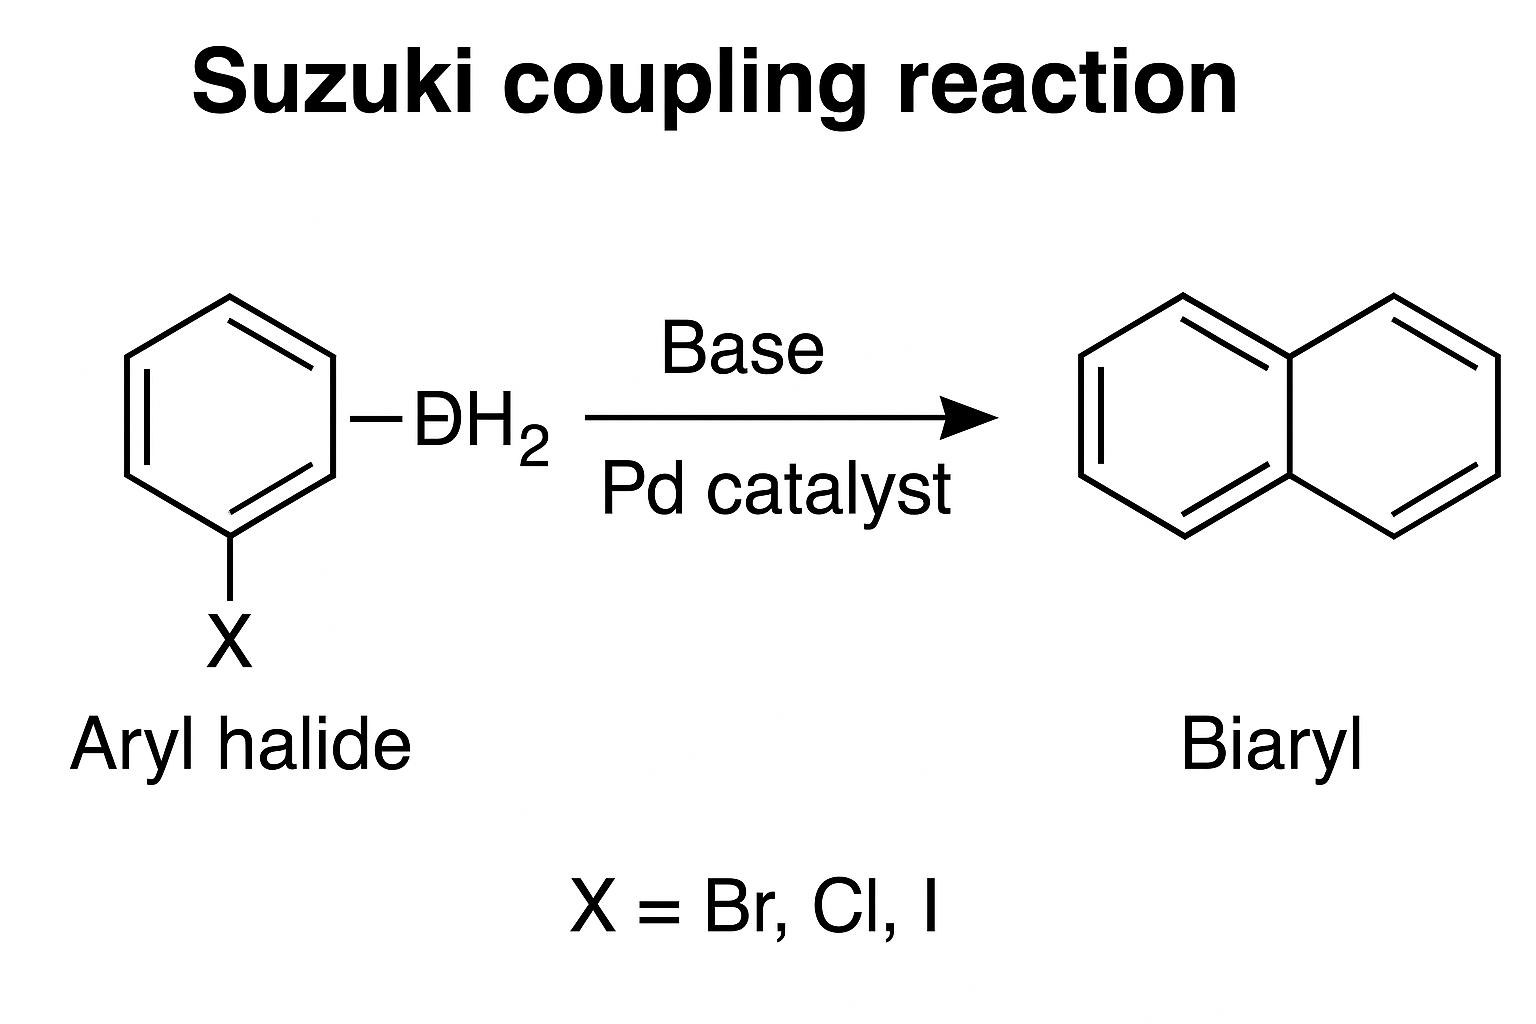
\includegraphics[width=0.5\linewidth]{suzuki_diagram.png}
    \caption{Representation of a Suzuki coupling reaction.}
\end{figure}

Even though the reaction is well known, figuring out the best conditions to run it, like which ligand, base, or solvent to use,  still takes a lot of work. There are so many possible combinations that testing them all by hand would take forever. That’s why machine learning and optimization tools are starting to get used in chemistry.

Bayesian Optimization is one of those tools. Instead of testing every setup, it uses math to predict which experiments are most likely to work well. Then it tests those and keeps learning from the results. We used a version of this called EDBO (Experimental Design via Bayesian Optimization), which was made specifically for chemistry. It’s designed to help find high-yield reactions faster and with fewer experiments.

To get meaningful results, the data going into the model still needs to make sense chemically. For example, steric effects how crowded or bulky a molecule is can seriously affect how well the reaction works. If a ligand or base is too bulky, it might block the catalyst or slow down the reaction. On the other hand, some bulk can actually help make the reaction more selective. Electronic effects are also important: electron-rich or electron-poor groups on the nucleophile or electrophile can speed up or slow down the reaction depending on how they interact with the catalyst. We also had to think about reactivity and stability some boronic acids are more reactive but degrade quickly, and some aryl halides are too unreactive under mild conditions. Solvent choice matters too; a good solvent helps everything dissolve properly and creates a stable environment for the catalyst. Poor solvent choice can shut down the reaction completely.

All of these chemical factors influence yield, and if the dataset doesn’t capture that — or includes unrealistic combinations — it makes it harder for the model to learn useful patterns. Understanding what makes a good reaction setup helped us better interpret the data and figure out how to use the model more effectively.


\section{Methods}
To use EDBO with new datasets, we first had to clean up the Perera dataset by making an entries column, and renaming all the Ligand values of None to Empty, as that messed up the GPyTorch Bayesian Optimization model the EDBO library used under the hood. 

Once we had all the data parsed, we used One Hot Encoding (OHE) to encode all the columns used by the model that didn’t have numerical values. An example of OHE is if we have a column in a database with addresses, instead of having the value as a string, we can give each row a column with the address and fill that value in with a 1 or 0 depending on if the entry’s address is or is not that column address value.

The reason we have to encode these columns is due to the fact that Bayesian Optimization can’t use string values in its calculation, only numbers. The reason OHE was chosen as the encoding method was that other encoding methods would've taken longer to implement. Once we had the dataset ready, we had to choose the acquisition function for Bayesian Optimization to use in its decision making, such as expected improvement, probability of improvement, Thompson sampling, etc. In the end, we chose expected improvement, as across the testing we did, and the results from the parent paper of EDBO, it seemed to perform the best in finding the highest yield consistently, and with a reasonable amount of batches. 

Then we made tweaks to the length-scale prior to make the model less certain of reaction areas it hadn't explored, the noise prior to introduce more randomness into the acquisition function, and increasing noise constraints of the model to give the noise more of an impact in the function's decision making, the model was now much more exploratory of unknown reaction areas, versus exploitative where it chooses slight variations on results that did well previously. These changes to the model were done as the default priors made the model too exploitative and it would never find the best result

In the end, using the expected improvement acquisition function, and the modified model priors, we ended up running 30 Bayesian Optimization instances that each ran for 15 batches with a batch size (how many experiments it would test per round) of 5. This meant that for each run we did, we performed a simulated 2,250 chemical experiments. However, many of these experiments were duplicates so our real experiments ran between 400-500 for each round of Bayesian Optimization in this dataset of 5761 experiments. 

We ran many instances of Bayesian Optimization with different features from the dataset included. The reason being that the performance of the model varied from features included, often with more data included ruining the Bayesian Optimization’s performance. One of the suspected reasons for this is that the simplified info that OHE provides makes the model produce false links in the data, a problem that would have likely been fixed if we would’ve used a different encoding method more oriented towards chemistry like Mordred or DFT encoding. 

\begin{figure}
    \centering
    \begin{subfigure}{0.49\textwidth}
        \centering
        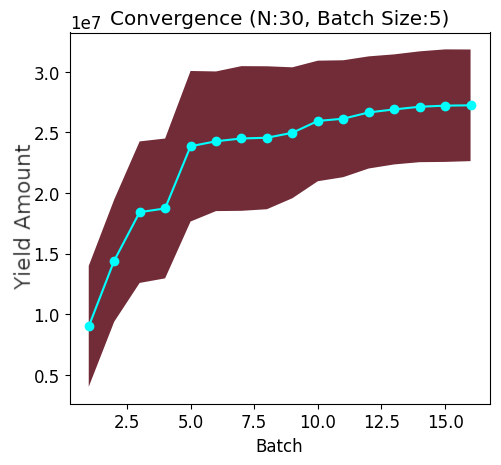
\includegraphics[width = \textwidth]{graph1.png}
        \caption{2 Inputs}
    \end{subfigure}
    \begin{subfigure}{0.49\textwidth}
        \centering
        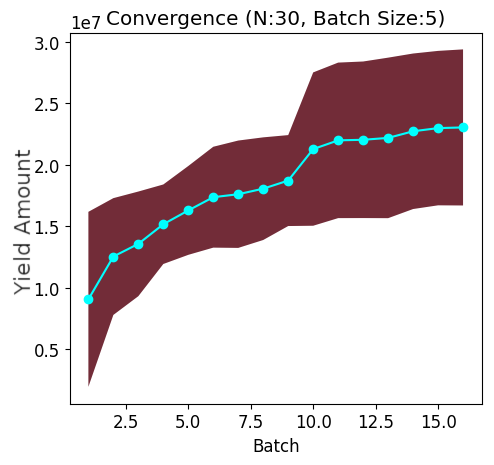
\includegraphics[width = \textwidth]{graph2.png}
        \caption{5 Inputs}
    \end{subfigure}
    \caption{(a) reaches high yield in fewer batches than (b).}
\end{figure}

This would’ve likely helped as the parent paper for EDBO compared the performance of each encoding method and found that DFT was the best, followed by Mordred, followed by OHE. This is why we think including less data improved the model as it had less data to make false correlations and didn’t have the context as to what that data actually meant, information that would’ve likely prevented it from making false correlations.

In the end, the main variable in our experimentation was which features from the data we included. These varied from which reactants were used, to what ligands were chosen. Even different solvents were included in the database. 

\section{Results}
We did not test all feature permutations from the dataset, but various features were tested to give a good idea on which provided the highest average yield at the end. Our final results show the mean of the Bayesian Optimization runs that used those features.
\begin{figure}[H]
    \centering
    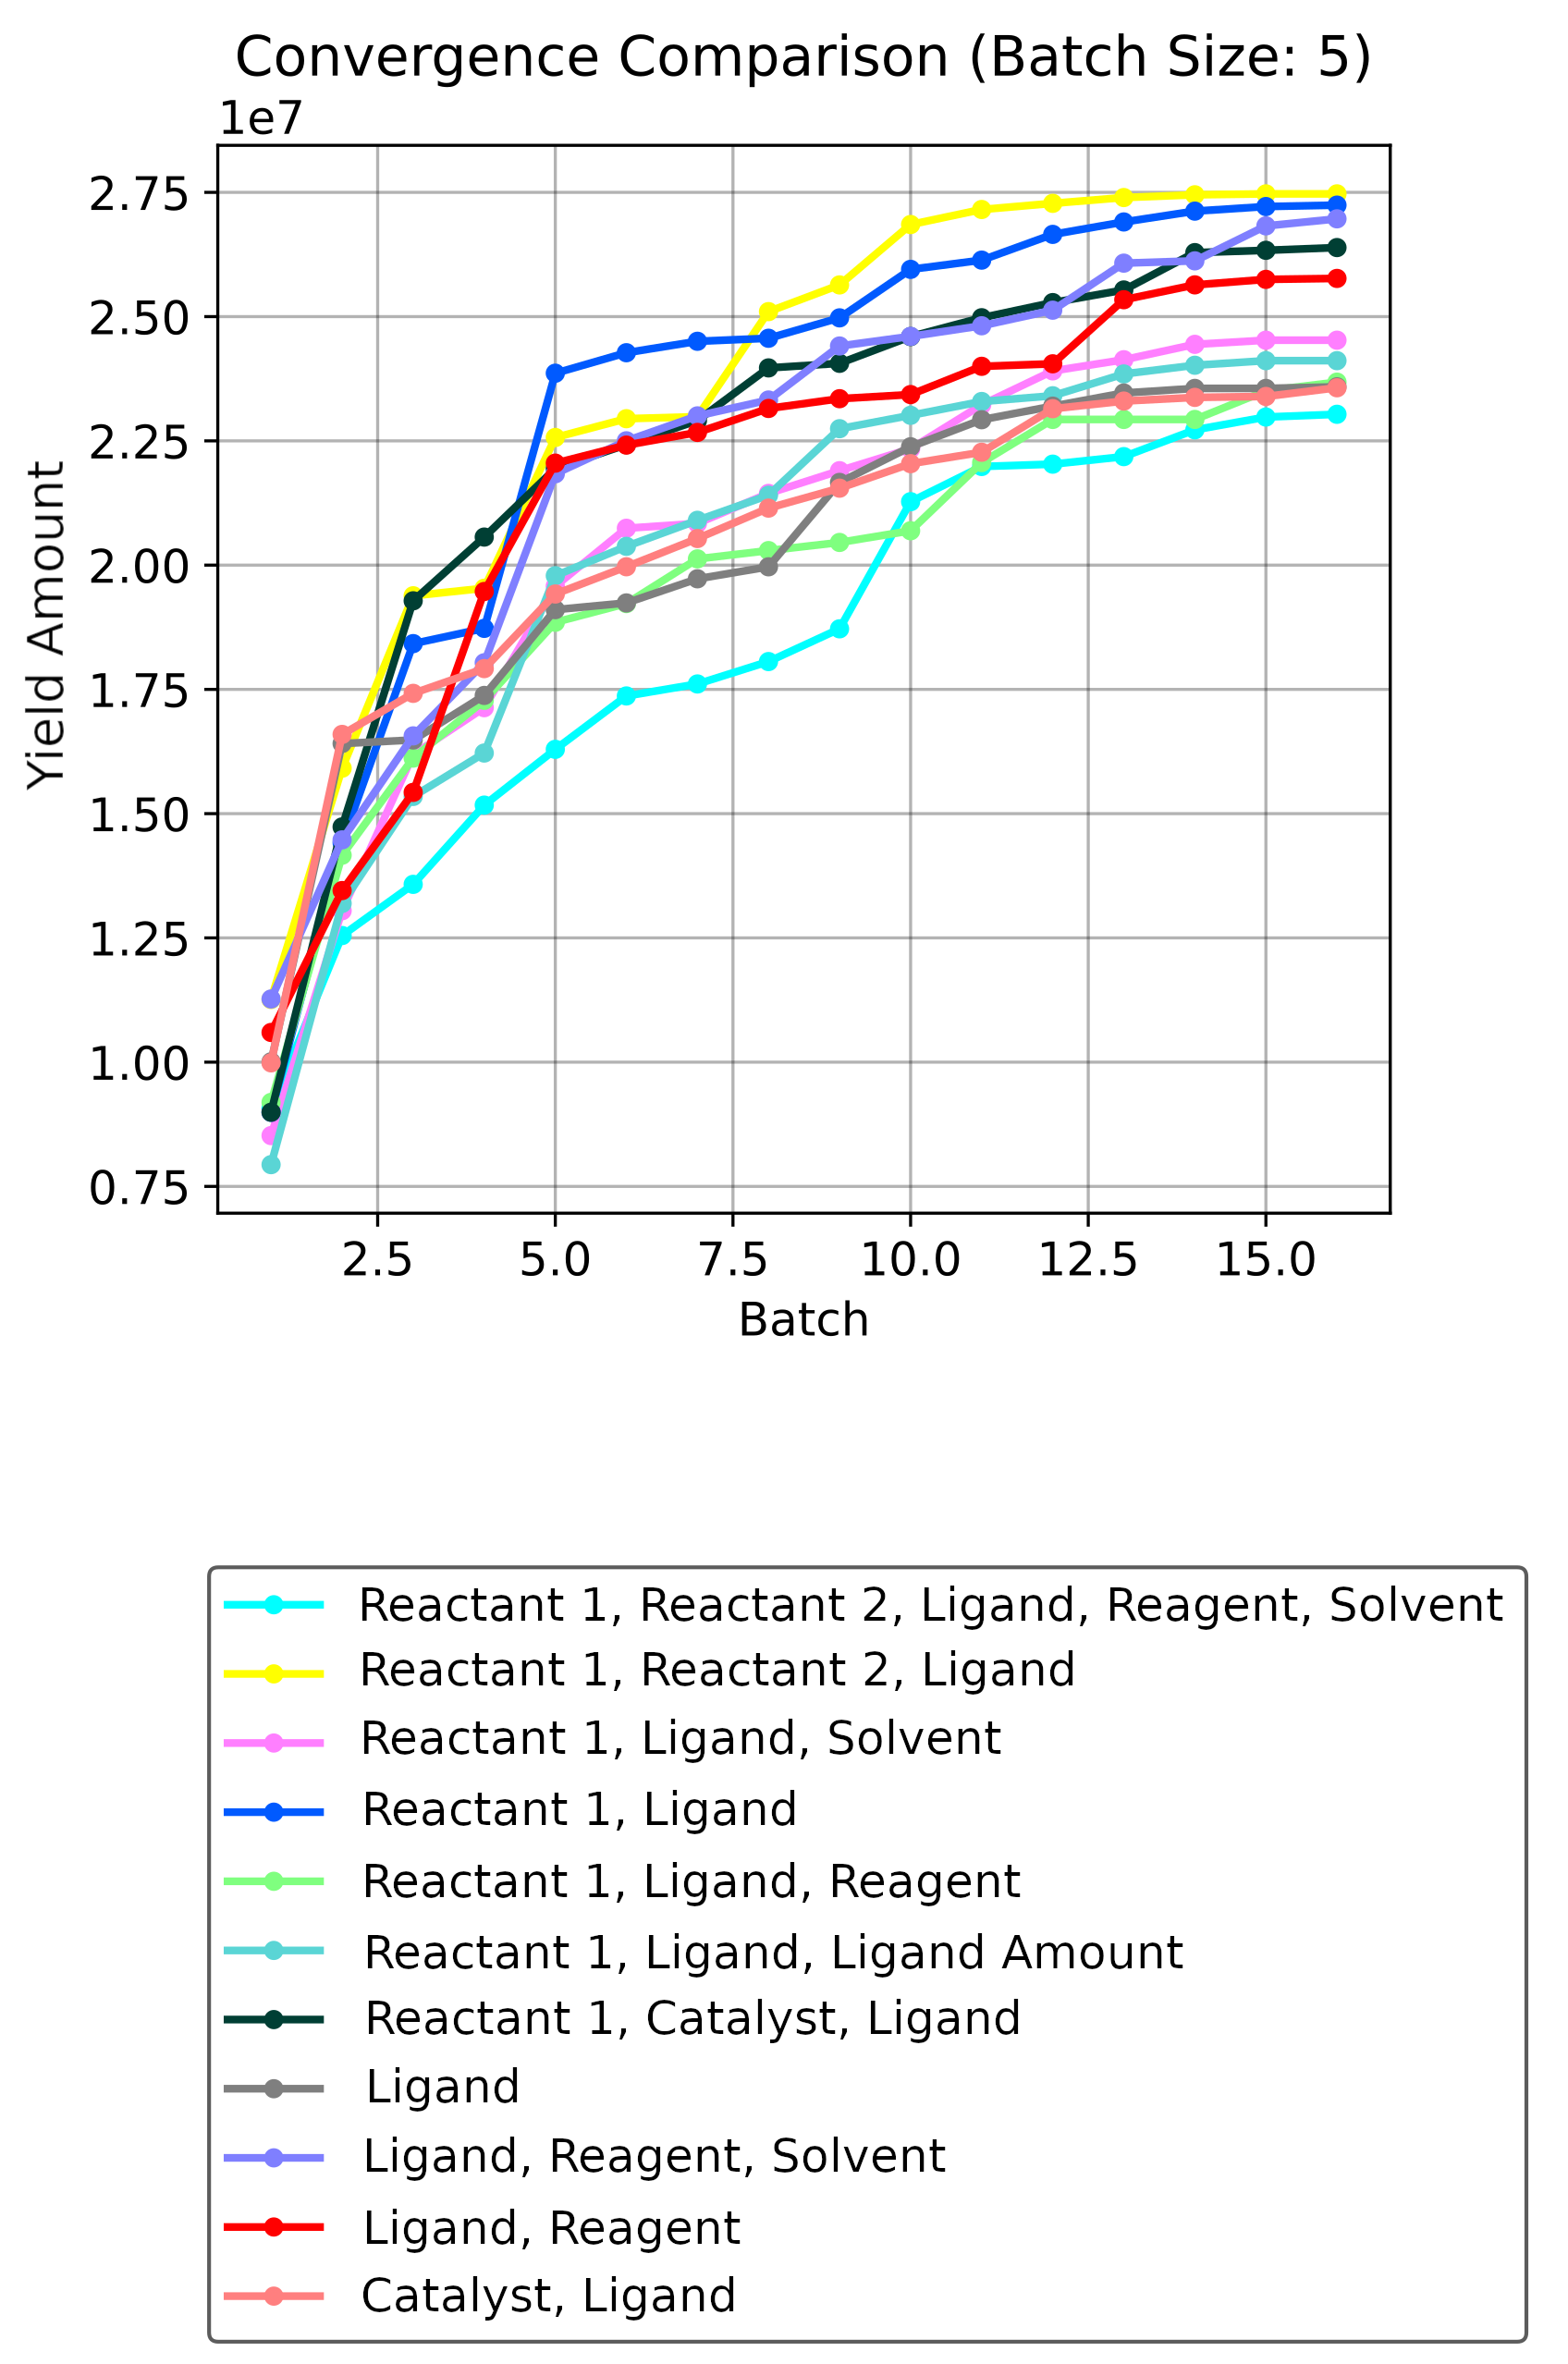
\includegraphics[width=0.75\linewidth]{final_graph.png}
    \caption{Graph of all the means of different data combinations.}
\end{figure}

In the end, we can see having the data from the two reactants used (Reactant\_1\_Name, Reactant\_2\_Name) and the data from the ligands used (Ligand\_Short\_Hand) produced the highest observed mean of all the different combinations of data.

We can also see the problem referenced earlier in the methods where more data given to the Bayesian Optimization model seemed to worsen its performance as the first entry in the legend, that gave the model the most data from each experiment, had the worst final mean of all the data combinations.

Even with the strange behavior of the model with OHE encoded data, nearly all of these only ran roughly roughly 400 experiments to find the maximum. The dataset came from a paper targeting optimization and they had a dataset size of 5,761. To interpret these results, we managed to find the highest grossing experiment in nearly all of these experiments with roughly 6.9\% of the experiments ran compared to the real life bulk testing to optimize.

Ignoring the fact we used a dataset that used bulk testing to optimize, we’ve also ran experiments on datasets as small as 500 experiments that used computers to optimize for their highest yield and we found we could consistently find the highest value in as few as 70 experiments on average, consistently.

\section{Future Work}
While we faced some challenges during the project, each of them helped us better understand both the potential and limits of applying Bayesian Optimization to chemistry. We weren’t able to test reactions in a lab and with only four weeks, even if we had access, there wouldn’t have been time to generate meaningful data. Still, this helped us focus on the computational side and explore how far we could go with modeling alone. In the future, combining this approach with actual lab work would let us test and refine our predictions.

Early on, we also spent time fixing broken code and updating outdated dependencies in the EDBO repo. This slowed things down initially, but in the end, it gave us a deeper understanding of the system and how it works under the hood. With more time, we’d like to add features like multi-objective optimization (e.g., balancing yield, cost, and time), DFT descriptor integration with Psi4, and more user-friendly interfaces that make the tool accessible to people with less coding experience.

One interesting direction for future work is exploring how human error affects experimental data. Real chemical reactions aren’t perfect — small measurement differences or technique changes can lead to inconsistent results. Since BO depends on clean data, we’d like to find ways to either detect noisy inputs or make the model more flexible in dealing with that kind of variability.

Lastly, we’d aim to improve the model’s speed. Some parts ran slower than expected, especially on a standard laptop. With faster hardware or more efficient code, the optimization could cover more ground and deliver results even quicker.

Even with the time limits and technical hurdles, this project showed us how powerful Bayesian Optimization can be in guiding reaction discovery. We were able to get the model working, test it on real-world datasets, and see clear potential for applying these tools in a lab setting. There’s a lot we’d still like to build — but we’re proud of what we accomplished.
\section{Conclusion}
In conclusion, our results demonstrate Bayesian Optimization is a highly efficient method for navigating complex chemical reaction spaces, particularly in situations where time, materials, or experimental access are limited. Despite our initial technical challenges, we showed that with a clean dataset and a few thoughtful adjustments, the model could identify high-yielding conditions with far fewer trials than a traditional workflow would require (as shown in the paper by B. Shields). This not only reduces cost and time but also makes the optimization process more accessible. While data quality, encoding methods, and computing power still pose some limitations, our project illustrates Bayesian Optimization is not just a theoretical tool—it is practical, scalable, and usable even by those with limited coding or machine learning experience.


\begin{thebibliography}{99}

\bibitem{1}
Perera, D.; Tucker, J. W.; Brahmbhatt, S.; Helal, C. J.; Chong, A.; Farrell, W.; Richardson, P.; Sach, N. W. A platform for automated nanomole-scale reaction screening and micromole-scale synthesis in flow. Science 2018, 359 (6374), 429–434. https://doi.org/10.1126/science.aap9112

\bibitem{2}
Shields, Benjamin J. “b-shields/edbo: Experimental Design via Bayesian Optimization.” Accessed July, 2025. https://github.com/b-shields/edbo.

\bibitem{3}
Coley, C. W.; Rogers, L.; Green, W. H.; Jensen, K. F. Computer-Assisted Retrosynthesis Based on Molecular Similarity. ACS Cent. Sci. 2017, 3, 1237–1245. https://doi.org/10.1021/acscentsci.7b00355

\bibitem{4}
Shields, Benjamin J., Jason Stevens, Jun Li, et al. “Bayesian Reaction Optimization as a Tool for Chemical Synthesis.” Nature 590, no. 7844 (2021): 89–96. https://doi.org/10.1038/s41586-021-03213-y.

\end{thebibliography}


\end{document}
